\documentclass{report}

\usepackage[francais]{babel}
\usepackage{ucs}
\usepackage[utf8x]{inputenc}
\usepackage{titlesec}
\usepackage{graphicx}
\usepackage{amssymb}
\usepackage{amsmath}
\usepackage{dsfont}



\title{\textbf{Projet de statistiques}}
\author{{Maxime \bsc{Peterlin} - Gabriel \bsc{Vermeulen} }\\\\{ENSEIRB-MATMECA, Bordeaux}}
\date{28, avril 2014}


\begin{document}


\maketitle

\tableofcontents

\chapter{Autour des variables aléatoires gaussiennes}
	\section{Variables aléatoires gaussiennes réelles}
		\subsection{Densité de probabilité d'une variable aléatoire gaussienne de de moyenne $\mu$ et de variance $\sigma^2$}
			La densité de probabilité d'une loi normale de moyenne 0 et de variance 1 est :
			\[f(x) = \frac{1}{\sqrt{2\pi}} \cdot exp(-\frac{x^2}{2}) \]
			Pour obtenir la densité de probabilité d'une variable aléatoire gaussienne de de moyenne $\mu$ et de variance $\sigma^2$, on effectue le changement de variable $y = \frac{x-\mu}{\sigma}$ :
			\[\int f(x)dx = \int \frac{1}{\sqrt{2\pi}} \cdot exp(-\frac{x^2}{2})dx = \int \frac{1}{\sqrt{2\pi}} \cdot exp(-\frac{(y-\mu)^2}{2\cdot \sigma^2})\frac{dy}{\sigma} = \int f(y)dy \]
			Ainsi, on a la densité de probabilité $f(y)$ recherchée :
			\[f(y) = \frac{1}{\sqrt{2\pi \sigma}} \cdot exp(-\frac{(y-\mu)^2}{2\cdot \sigma^2}) \]
			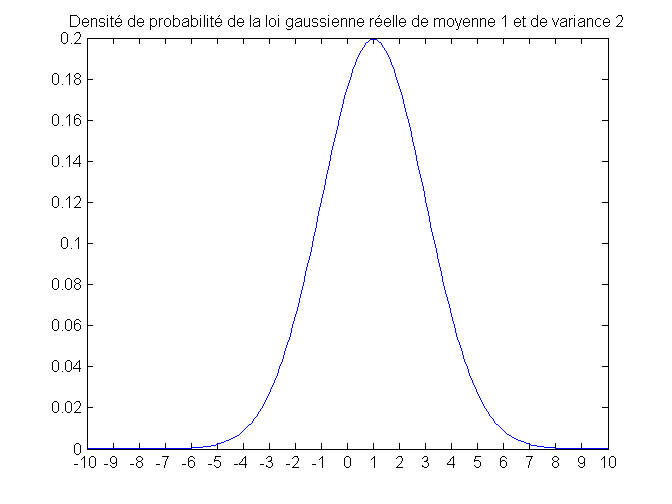
\includegraphics[scale=0.7]{sources/Q211.png} 
		\subsection{Histogramme de 100 réalisations de la loi $\mathcal{N}_{\mathbb{R}}(5, 1)$}
			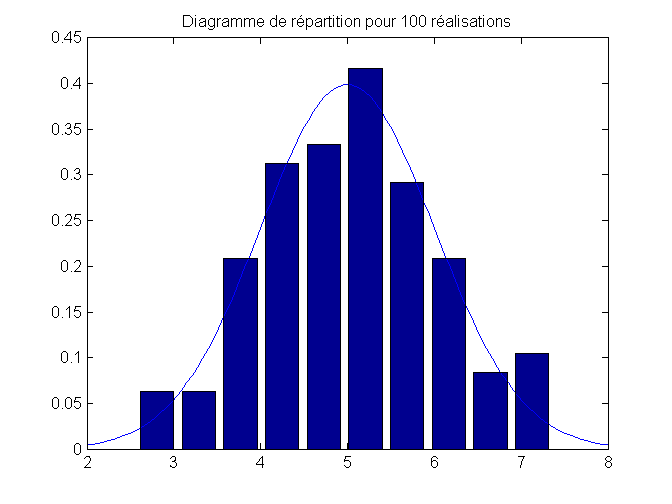
\includegraphics[scale=0.7]{sources/Q212-1.png} \\
			La proportion empirique entre [$\mu$ − $\sigma$, $\mu$ + $\sigma$] est égale à 63. \\
			La proportion empirique entre [$\mu$ − 3 $\sigma$, $\mu$ + 3 $\sigma$] est égale à 100. \\
		\subsection{Histogramme de 1000 réalisations de la loi $\mathcal{N}_{\mathbb{R}}(5, 1)$}
			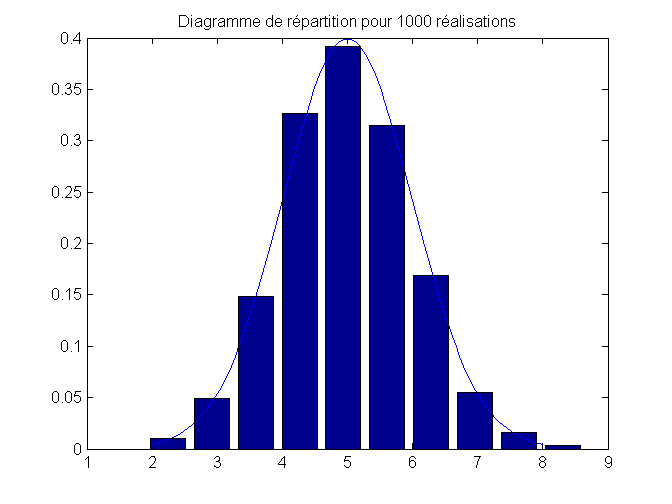
\includegraphics[scale=0.7]{sources/Q212-2.png} \\
			La proportion empirique entre [$\mu$ − $\sigma$, $\mu$ + $\sigma$] est égale à 713. \\
			La proportion empirique entre [$\mu$ − 3 $\sigma$, $\mu$ + 3 $\sigma$] est égale à 998. \\
			On remarque que plus le nombre de réalisations est grand, moins ces valeurs empiriques sont aléatoires, et plus elles convergent vers les valeurs théoriques vues en cours. \\

	\section{Variables aléatoires gaussiennes vectorielles}
		\subsection{Fonction caractéristique de la variable $t^TX$}
			On a 
			\[\Phi_{t^TX}(u) = \mathbb{E}[e^{iut^TX}] = \mathbb{E}[e^{iu\sum\limits_{k=1}^{n}t_kX_k}] \]
		\subsection{Montrons que les $X_1, \ldots, X_n$ sont indépentantes}
			En se servant du lemme donné, si 
			\[\mathbb{E}[e^{i\sum\limits_{k=1}^{n}t_kX_k}] = \prod\limits_{k=1}^{n}\mathbb{E}[e^{it_kX_k}]\]
			alors les variables aléatoires $X_1, \ldots, X_n$ seront indépendantes.
			Soit $X \sim \mathcal{N}_{\mathbb{R}^\mathbb{N}}(\mu, \sigma^2)$ et $Y \sim \mathcal{N}_{\mathbb{R}^\mathbb{N}}(O, I)$, on a la relation suivante entre $X$ et $Y$ :
			\[ X = m + \sigma Y \]
			On en déduit que
			\[ \Phi_X(u) = \mathbb{E}[e^{iuX}] = \mathbb{E}[e^{iu(m+\sigma Y)}] = e^{ium}\mathbb{E}[e^{iu\sigma Y}] = e^{ium-\frac{\sigma^2 u^2}{2}} \]
			Comme $X \sim \mathcal{N}_{\mathbb{R}^\mathbb{N}}(O, I)$, alors $t^TX \sim \mathcal{N}_{\mathbb{R}^\mathbb{N}}(O, \sum\limits_{k=1}^{n}t_k^2)$.\\
			Ainsi $\Phi_{t^TX}(u) = e^{-\frac{u^2}{2}\sum\limits_{k=1}^{n}t_k^2}$ et $\Phi_{t^TX}(1) = e^{-\frac{1}{2}\sum\limits_{k=1}^{n}t_k^2}$.\\
			De plus, $\Phi_{X_k}(t_k) = e^{-\frac{t_k^2}{2}} = \mathbb{E}[e^{it_kX_k}] $, donc $\prod\limits_{k=1}^{n}\Phi_{X_k}(t_k) = \Phi_{t^TX}(1) = \mathbb{E}[e^{i\sum\limits_{k=1}^{n}t_kX_k}] $.\\
			On a bien montré que 
			\[\mathbb{E}[e^{i\sum\limits_{k=1}^{n}t_kX_k}] = \prod\limits_{k=1}^{n}\mathbb{E}[e^{it_kX_k}]\]
			Donc les variables aléatoires $X_1, \ldots, X_n$ sont indépendantes.
		\subsection{Densité de probabilité de la loi $\mathcal{N}_{\mathbb{R}^n}(0, I)$}
			On a $\forall k$, $X_k \sim \mathcal{N}_{\mathbb{R}}(0, 1)$ indépendantes, ainsi
			\[ f(X) = f(X_1, \ldots X_n) = \prod\limits_{k=1}^{n}f_k(X_k) = (\frac{1}{\sqrt{2\pi}})^ne^{-\frac{1}{2}\sum\limits_{k=1}^{n}x_k} \]
		\subsection{Densité de probabilité de la loi $\mathcal{N}_{\mathbb{R}^n}(\mu, \Gamma)$}
		\subsection{Montrons que les composantes d'un vecteur gaussien sont indépendantes si et seulement si sa matrice de covariance est diagonale}
			Si les composantes d'un vecteur gaussien sont indépendantes, alors $\forall i \neq j$ on a $COV(X_i, X_j) = 0$, ainsi, la matrice de covariance a tous ses éléments non diagonaux qui sont nuls. Cette dernière est donc diagonale.\\
			Réciproquement, si la matrice de covariance est diagonale, alors :
			\[ f_k(X_k) = \frac{1}{\sqrt{2\pi}\sigma_k}e^{-\frac{1}{2}\sum\limits_{k=1}^{n}\frac{(x_1 - \mu_1)^2}{\sigma_k^2}} \]
			et
			\[f(X) = \frac{1}{\sqrt{2\pi}^n\prod\limits_{k=1}^{n}\sigma_k}e^{-\frac{1}{2}(x-\mu)^T\left[ 
				\begin{array}{ccc} 
					\sigma_1^2 & \cdots & 0 \\
					\vdots & \ddots & \vdots \\
					0 & \cdots & \sigma_n^2 \\
				\end{array} 
			\right]^{-1}(x-\mu)} = \frac{1}{\sqrt{2\pi}^n\prod\limits_{k=1}^{n}\sigma_k}e^{-\frac{1}{2}\sum\limits_{k=1}^{n}\frac{(x_k - \mu_k)}{\sigma_k^2}} \]
			On a bien $\prod\limits f_k(X_k) = f(X)$, les variables sont donc indépendantes.

		\subsection{Tracé de la densité de la loi $\mathcal{N}_{\mathbb{R}^2}(\mu, \Gamma)$}
			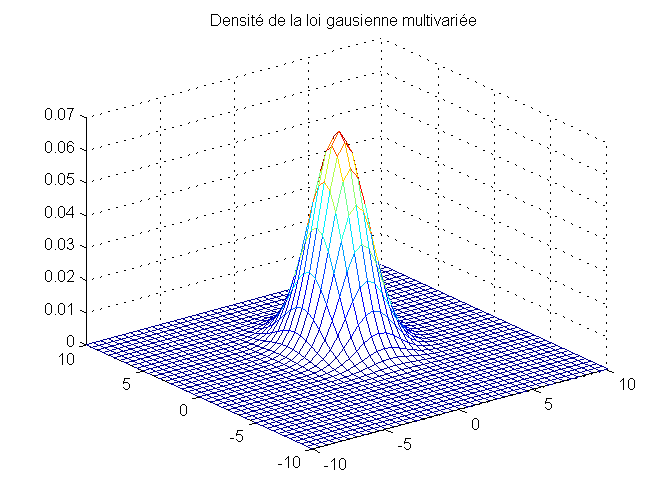
\includegraphics[scale=0.7]{sources/Q222-1.png}
		\subsection{Histogramme de 1000 réalisations de la loi $\mathcal{N}_{\mathbb{R}^2}(\mu, \Gamma)$}
			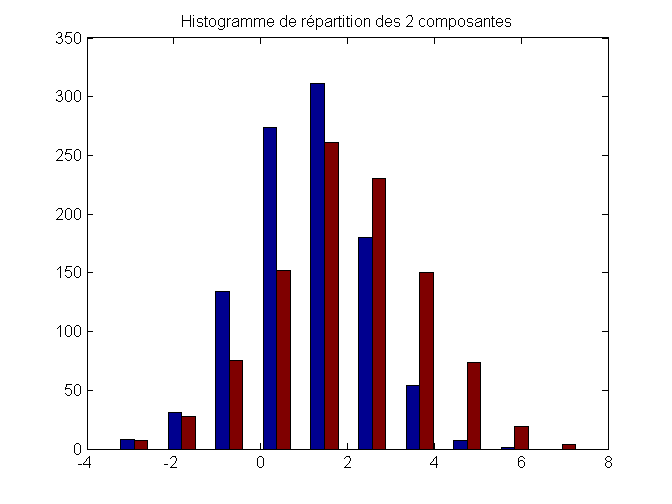
\includegraphics[scale=0.7]{sources/Q222-2.png}
		\subsection{Montrons que $X \sim \mathcal{N}_{\mathbb{R}^d}(0, I) \Rightarrow UX \sim \mathcal{N}_{\mathbb{R}^d}(0, I), \forall U \in \mathbb{O}_d(\mathbb{R})$}
			On a $UX = [a_1, \ldots, a_d]$, avec $\forall k, a_k = \sum\limits_{i=1}^d u_{ki}X_i$.\\
			Calculons l'espérance de ce vecteur : 
			\[ \mathbb{E}[UX] = \mathbb{E}\left[ [\sum\limits_{i=1}^d u_{1i}X_i, \ldots, \sum\limits_{i=1}^d u_{di}X_i]\right] = \left[ \sum\limits_{i=1}^d u_{1i}\mathbb{E}[X_i], \ldots, \sum\limits_{i=1}^d u_{di}\mathbb{E}[X_i]\right] = 0\]car $\forall i, \mathbb{E}[X_i] = 0$.\\
			\\
			Calculons à présent sa variance
			\[ Var[UX] = \mathbb{E}[(UX)(UX)^T] = \mathbb{E}[U X X^T U^T] = U \mathbb{E}[XX^T]U^T \]
			Nous savons également que
			\[ Var[X] = \mathbb{E}[X X^T] - \mathbb{E}^2[X] = \mathbb{E}[X X^T] = I \]
			Ainsi, $Var[X] = UU^T = I$, car $U \in \mathbb{O}_d(\mathbb{R})$.\\
			Nous avons donc montré que $X \sim \mathcal{N}_{\mathbb{R}^d}(0, I) \Rightarrow UX \sim \mathcal{N}_{\mathbb{R}^d}(0, I), \forall U \in \mathbb{O}_d(\mathbb{R})$.

		\subsection{Histogramme de 1000 réalisations du vecteur $UX$}
			\begin{center}
				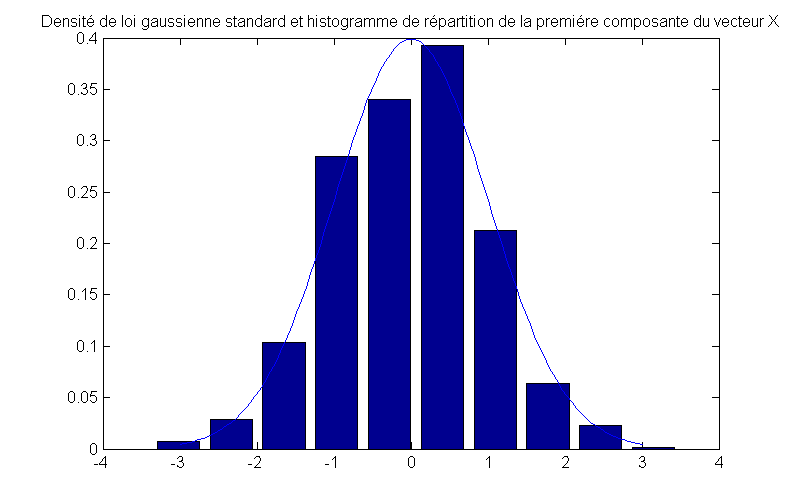
\includegraphics[scale=0.7]{sources/Q223-1.png}
				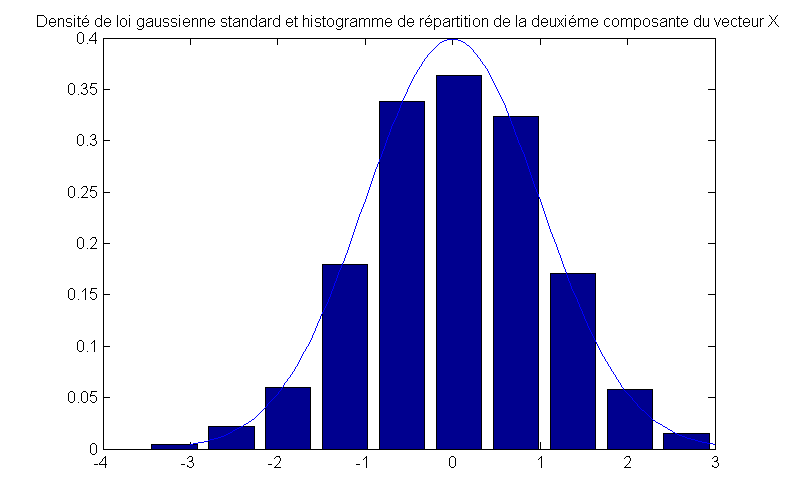
\includegraphics[scale=0.7]{sources/Q223-2.png}
			\end{center}
		\subsection{Démonstration et vérification expérimentale du caractère gaussien d'un vecteur donné}
			On a $X \sim \mathcal{N}_{\mathbb{R}}(0, 1)$.\\
			On pose $\textbf{X} = [X_1, X_2]^T$, avec $X_1 = X et X_2 = ZX$.
			$Z$ est une variable aléatoire indépendante de X de loi uniforme sur l'intervalle $\{-1, 1\}$\\
			\\
			On veut montrer que $X_1$ et $X_2$ suivent des lois gaussiennes.\\
			Il est évident que c'est le cas pour $X_1$, montrons le pour $X_2$.
			La densité de probabilité que suit Z est
			\[ f_Z(x) = \frac{1}{2}\delta(x+1) + \frac{1}{2}\delta(x-1) \]
			La densité de probabilité que suit X est
			\[ f_X(x) = \frac{1}{\sqrt{2\pi}} exp(-\frac{x^2}{2}) \]
			La densité de probabilité que suit ZX est la convolution de leur densité respective.
			\[ f_{ZX}(x) = (f_X \ast f_Z)(x) = [f \ast (\frac{1}{2}\delta_{-1} + \frac{1}{2}\delta_{1})](x) = \frac{1}{2}f(x+1) + \frac{1}{2}f(x-1) \]
			La fonction caractéristique d'une variable $X \sim \mathcal{N}_{\mathbb{R}}(0, 1)$ est 
			\[ \Phi_X(u) = \mathbb{E}[e^{iuX}] = e^{-\frac{u^2}{2}} \]
			Ainsi
			\begin{align*}
				\Phi_{ZX}(u) &= \mathbb{E}[e^{iuZX}] = \int_{\mathbb{R}}f_{ZX}(y)e^{ity}dy = \int_{\mathbb{R}}(\frac{1}{2}f_X(x+1) + \frac{1}{2}f_X(x-1))e^{ity}dy\\
				&= \int_{\mathbb{R}}\frac{1}{2}f(x+1)e^{ity}dy + \int_{\mathbb{R}}\frac{1}{2}f(x-1)e^{ity}dy\\
				&= \frac{1}{2}e^{-\frac{u^2}{2}} + \frac{1}{2}e^{-\frac{u^2}{2}} = e^{-\frac{u^2}{2}}
			\end{align*}
			car $f_X$ suit une loi $\mathcal{N}_{\mathbb{R}}(0, 1)$.\\
			Nous avons donc prouvé que $X_2 \sim \mathcal{N}_{\mathbb{R}}(0, 1)$.\\
			A présent, nous allons voir si le vecteur $\textbf{X}$ est gaussien ou non.\\
			Si le vecteur $\textbf{X}$ était gaussien, il aurait la fonction caractéristique suivante :
			\[ \Phi_{\textbf{X}}(u) = e^{-\frac{u^2}{2}} \]
			Calculons sa fonction caractéristique.
			\[ \Phi_{\textbf{X}}(u) = \mathbb{E}(e^{i<u,X>}) = \int_{\mathbb{R}}\int_{\mathbb{R}}f_{\textbf{X}}(x,z)e^{iu_1x + iu_2xz}dxdz \]
			$X$ et $ZX$ n'étant pas indépendant, on ne peut retrouver la bonne fonction caractéristique.\\
			Le vecteur $\textbf{X}$ n'est donc pas gaussien. \\
			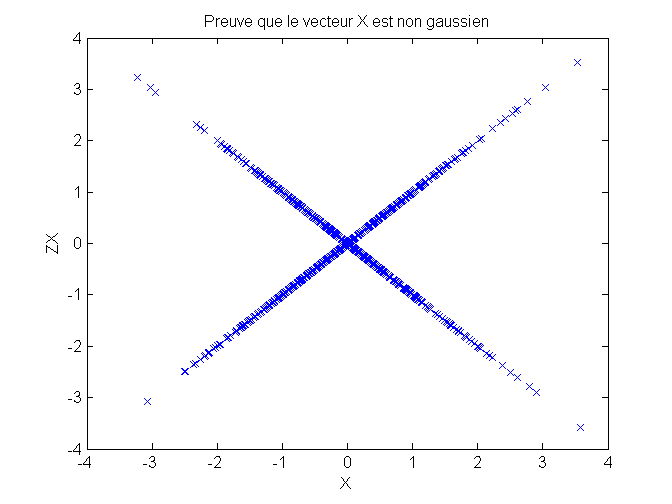
\includegraphics[scale=0.7]{sources/Q224.png}
	\section{Variables aléatoires gaussiennes complexes}
		\subsection{Variance et densité de probabilité de $Z \sim \mathcal{N}_{\mathbb{C}}(\mu, \sigma^2)$}
			Calculons la variance de la variable aléatoire $Z = X + iY$.
			\begin{align*}
				V[Z] &= \mathbb{E}\left[|Z-\mathbb{E}[Z]|^2\right] = \mathbb{E}\left[|Z|^2+|\mathbb{E}[Z]|^2-2\Re(Z\overline{\mathbb{E}[Z]})\right]\\
				&= \mathbb{E}[|Z|^2]-|\mathbb{E}[Z]|^2 = \mathbb{E}[|X+iY|^2]-|\mathbb{E}[X+iY]|^2\\ 
				&= \mathbb{E}[X^2+Y^2] - (\mathbb{E}^2[X] + \mathbb{E}^2[Y]) = Var[X] + Var[Y] = \sigma^2
			\end{align*}
			Calculons à présent la densité de probabilité de Z.\\
			On sait que X et Y sont indépendantes, ainsi
			\begin{align*}
				f_{XY}(X,Y) &= f_X(X)f_Y(Y)\\
				&= \frac{1}{\sqrt{2\pi}\frac{\sigma}{\sqrt{2}}}exp(-\frac{1}{2}\frac{(x-\Re(\mu))^2}{\frac{\sigma^2}{2}}) \cdot \frac{1}{\sqrt{2\pi}\frac{\sigma}{\sqrt{2}}}exp(-\frac{1}{2}\frac{(y-\Im(\mu))^2}{\frac{\sigma^2}{2}})\\
				&= \frac{1}{\sigma^2\pi}e^{-\frac{|z-\mu|^2}{\sigma^2}}
			\end{align*}
		\subsection{Histogramme de 1000 réalisations de la loi $\mathcal{N}_{\mathbb{C}}(0, 1)$}
		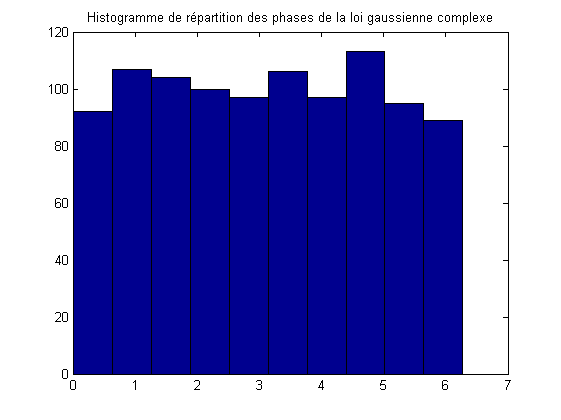
\includegraphics[scale=0.7]{sources/Q232.png}
	\section{Théorème de la limite centrale}
		\subsection{Loi de $W_n$ lorsque $X_k \sim \mathcal{N}_{\mathbb{R}}(\mu, \sigma^2)$}
			On sait que $\forall k, X_k \sim \mathcal{N}_{\mathbb{R}}(0, 1)$, de plus, on a 
			\[ W_n = \frac{1}{\sqrt{n}} \sum\limits_{k=1}^n \frac{X_k - \mu}{\sigma} \]
			Nous cherchons la loi de $W_n$ en sachant que $\forall k, X_k$ suit une loi normale. \\
			Posons 
			\[ Y_k = \frac{X_k - \mu}{\sqrt{n}\sigma} \]
			Commençons par calculer l'espérance de $Y_k$
			\[ \mathbb{E}[Y_k] = \mathbb{E}\left[ \frac{X_k - \mu}{\sqrt{n}\sigma} \right] = \frac{\mathbb{E}[X_k] - \mu}{\sqrt{n}\sigma} = 0 \]
			Calculons à présent la variance de $Y_k$
			\[ Var[Y_k] = Var\left[ \frac{X_k - \mu}{\sqrt{n}\sigma} \right] = \frac{1}{n\sigma^2}Var[X_k-\mu] = \frac{1}{n\sigma^2}\sigma^2 = \frac{1}{n} \]
			Nous avons donc $Y_k \sim \mathcal{N}_{\mathbb{R}}(0, \frac{1}n{})$
			Ainsi
			\[ W_n = \sum\limits_{k=1}^n Y_k \sim \mathcal{N}_{\mathbb{R}}(0, \sqrt{\sum\limits_{k=1}^n\frac{1}{n}} = 1) \]
		\subsection{Histogramme de 1000 réalisations de la loi $W_n$ lorsque $X_k \sim \mathcal{N}_{\mathbb{R}}(\mu, \sigma^2)$}
			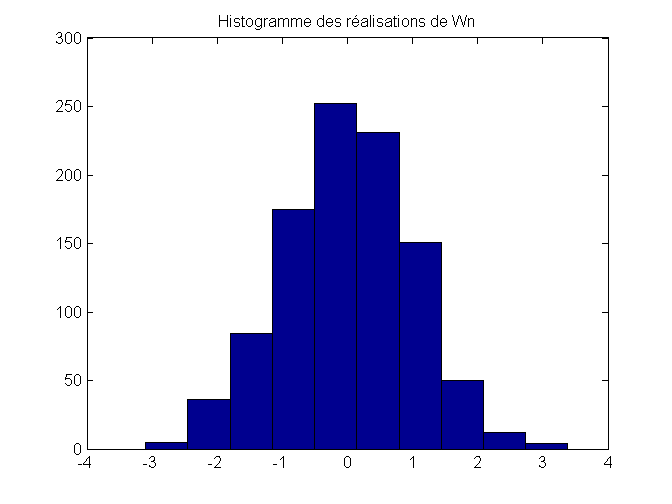
\includegraphics[scale=0.7]{sources/Q241.png}
		\subsection{Histogramme de 1000 réalisations de la loi $W_n$ lorsque $X_k \sim \mathcal{U}([0,1])$}
			\begin{center}
				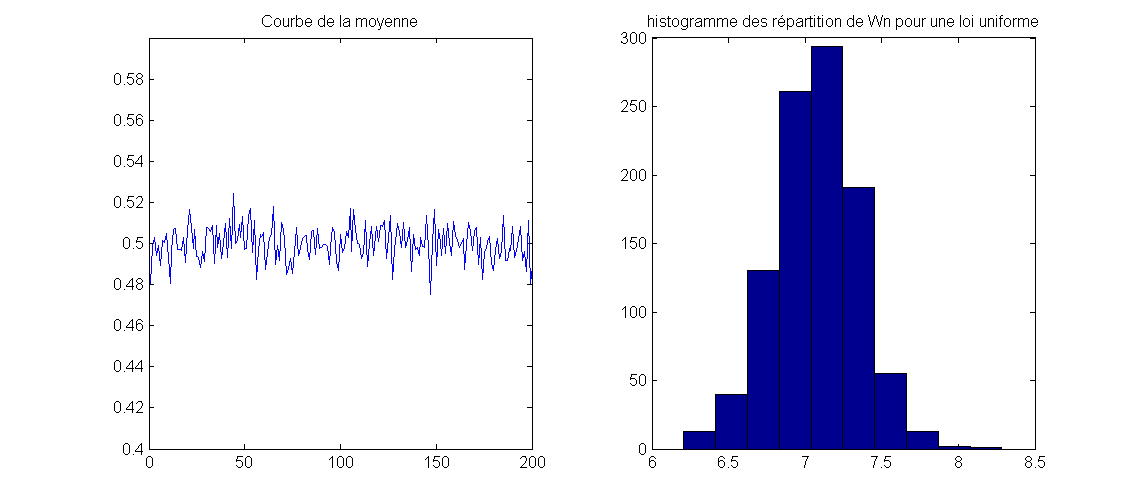
\includegraphics[scale=0.7]{sources/Q242-1.png}
			\end{center}
		Calcul de l'espérance et de la variance de $X_k, \forall k$
		\begin{align*}
			\mathbb{E}[X_k] &= \int\limits_0^1 x dx = \frac{1}{2}\\
			Var[X_k] &= \mathbb{E}[X_k^2] - \mathbb{E}^2[X_k] = \frac{1}{3} - \frac{1}{4} = \frac{1}{12}
		\end{align*}
		\subsection{Histogramme de 1000 réalisations de la loi $W_n$ lorsque $X_k \sim \mathcal{B}(\frac{1}{2}) $}
			\begin{center}
				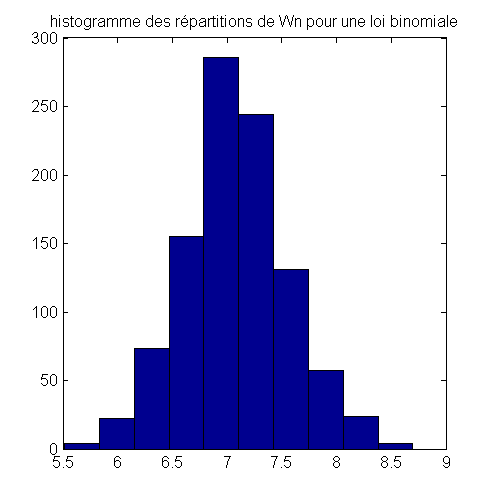
\includegraphics[scale=0.7]{sources/Q242-2.png}
			\end{center}
		Calcul de l'espérance et de la variance de $X_k, \forall k$
		\begin{align*}
			\mathbb{E}[X_k] &= p = \frac{1}{2}\\
			Var[X_k] &= p(1-p) = \frac{1}{2}
		\end{align*}
		
	\section{Loi du $\chi^2$}
		\subsection{Densité de probabilité d'une variable suivant une loi $\chi^2(n)$}
			Montrons par récurrence que la densité de probabilité de $Y \sim \chi^2(n)$ est
			\[ f_n(x) = \frac{x^{\frac{n}{2}-1}e^{-\frac{x}{2}}}{2^{\frac{n}{2}}\Gamma(\frac{n}{2})}\mathds{1}_\mathbb{R^+}(x) \]
			Tout d'abord, montrons le pour $n=1$. On a $Y=X^2$.\\
			Pour toutes fonctions $\phi$ bornée, on a :
			\begin{align*} 
				\mathbb{E}[\phi(y)] &= \mathbb{E}[\phi(x^2)] = \int_\mathbb{R} \phi(x^2)f_X(x)dx\\
				&= \int\limits_{-\infty}^{0} \phi(x^2)f_X(x)dx + \int\limits_0^{\infty} \phi(x^2)f_X(x)dx\\
				&= \int\limits_0^{\infty} \phi(x^2)f_X(-x)dx + \int\limits_0^{\infty} \phi(x^2)f_X(x)dx
			\end{align*}
			Posons le changement de variable $x=\sqrt{u}$, $dx=\frac{du}{2\sqrt u}$.
			\begin{align*} 
				\mathbb{E}[\phi(y)] &= \int\limits_0^{\infty} \phi(u)f_X(-\sqrt{u})\frac{du}{2\sqrt u} + \int\limits_0^{\infty} \phi(u)f_X(\sqrt{u})\frac{du}{2\sqrt u} \\
				&= \int\limits_0^{\infty} \phi(u)[f_X(-\sqrt{u}) + f_X(\sqrt{u})]\frac{du}{2\sqrt u}
			\end{align*}
			Ainsi, pour $Y=X^2$, la densité de probabilité s'exprime de la façon suivante :
			\[ f_Y(y) = \frac{1}{2\sqrt y}[f_X(-\sqrt{y}) + f_X(\sqrt{y})]\mathds{1}_\mathbb{R^+}(x) \]
			On en déduit donc que 
			\[ f_1(x) = \frac{x^{-\frac{1}{2}}}{2\sqrt{2\pi}}[e^{-\frac{x}{2}} + e^{-\frac{x}{2}}]\mathds{1}_\mathbb{R^+}(x) = \frac{x^{-\frac{1}{2}}e^{-\frac{x}{2}}}{\sqrt{2\pi}}\mathds{1}_\mathbb{R^+}(x) \]
			Supposons que la propriété soit vraie au rang $n$ et montrons le au rang $n+1$ :
			\begin{align*}
				f_{n+1}(x) &= f_{n}(x) \ast f_1(x) = \int_\mathbb{R} f_n(t)f_1(x-t)dt\\
				&= \frac{1}{2^{\frac{n+1}{2}}\Gamma(\frac{n}{2})\Gamma(\frac{1}{2})}e^{-\frac{x}{2}}\mathds{1}_\mathbb{R^+}(x)\int\limits_0^x t^{\frac{n}{2}-1}(x-t)^{-\frac{1}{2}}dt
			\end{align*}
			Posons le changement de variable $t = xu$, $dt = xdu$.

			\begin{align*}
				f_{n+1}(x) &= \frac{1}{2^{\frac{n+1}{2}}\Gamma(\frac{n}{2})\Gamma(\frac{1}{2})}e^{-\frac{x}{2}}\mathds{1}_\mathbb{R^+}(x)\int\limits_0^1 (xu)^{\frac{n}{2}-1}(x-xu)^{-\frac{1}{2}}du\\
				&= \frac{1}{2^{\frac{n+1}{2}}\Gamma(\frac{n}{2})\Gamma(\frac{1}{2})}e^{-\frac{x}{2}}\mathds{1}_\mathbb{R^+}(x)\int\limits_0^1 (xu)^{\frac{n}{2}-1}(x-xu)^{-\frac{1}{2}}xdu\\
				&= \frac{1}{2^{\frac{n+1}{2}}\Gamma(\frac{n}{2})\Gamma(\frac{1}{2})}e^{-\frac{x}{2}}x^{\frac{n+1}{2}-1}\beta(\frac{n}{2}, \frac{1}{2})\mathds{1}_\mathbb{R^+}(x)\\
				&= \frac{x^{\frac{n+1}{2}-1}e^{-\frac{x}{2}}}{2^{\frac{n+1}{2}}\Gamma(\frac{n+1}{2})}\mathds{1}_\mathbb{R^+}(x)
			\end{align*}
		\subsection{Moyenne et variance de la loi $\chi^2(n)$}
			Calculons l'espérance de $Y$
			\[ \mathbb{E}[Y] = \mathbb{E}[\sum\limits_{k=1}^n X_k^2] = \sum\limits_{k=1}^n\mathbb{E}[X_k^2] = \sum\limits_{k=1}^n Var[X_k] + \mathbb{E}^2[X_k] = n \]
			Calculons à présent la variance de $X^2$
			\[ Var[X^2] = \mathbb{E}[X_k^4] - \mathbb{E}^2[X_k^2] \]
			Déterminons l'expression de $\mathbb{E}[X_k^4]$
			\begin{align*}
				\mathbb{E}[X_k^4] &= \frac{1}{\sqrt{2\pi}}\int_\mathbb{R} x^4 e^{-\frac{x^2}{2}}dx = \frac{1}{\sqrt{2\pi}}\int_\mathbb{R} x^3 \cdot xe^{-\frac{x^2}{2}}dx\\
				&= \frac{1}{\sqrt{2\pi}}[-x^3 e^{-\frac{x^2}{2}}]_\mathbb{R}+\frac{1}{\sqrt{2\pi}}\int_\mathbb{R} 3x^2e^{-\frac{x^2}{2}}dx\\
				&= \frac{3}{\sqrt{2\pi}}\int_\mathbb{R} x \cdot xe^{-\frac{x^2}{2}}dx\\
				&= \frac{3}{\sqrt{2\pi}}[-x e^{-\frac{x^2}{2}}]_\mathbb{R}+\frac{3}{\sqrt{2\pi}}\int_\mathbb{R} e^{-\frac{x^2}{2}}dx\\
				&= 3 \cdot \int_\mathbb{R} \frac{1}{\sqrt{2\pi}}e^{-\frac{x^2}{2}}dx = 3
			\end{align*}
			Ainsi
			\begin{align*}
				\mathbb{E}[X_k^4] &= 3\\
				Var[X_k^2] &= \mathbb{E}[X_k^4] - \mathbb{E}^2[X_k^2] = 3-1 = 2
			\end{align*}
			On a donc $Var[Y^2] = \sum\limits_{k=1}^n Var[X_k^2] = 2n$, car les variables sont indépendantes.
		\subsection{Tracé de la densité de probabilité de la loi $\chi^2(n)$}
			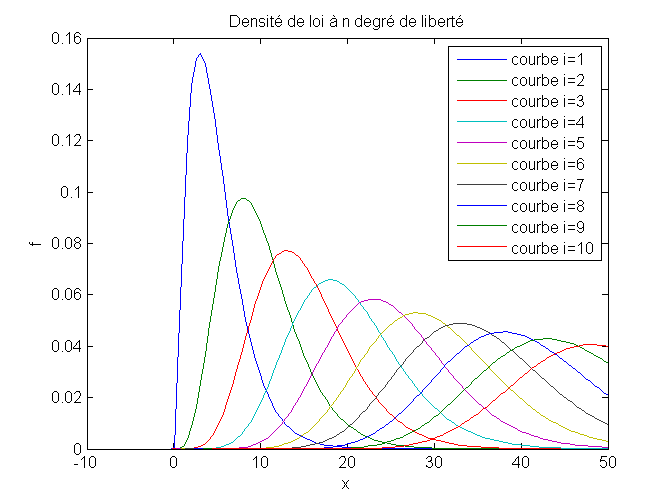
\includegraphics[scale=0.7]{sources/Q252.png} \\
			Lorsque n est grand, la densité est beaucoup plus étandue.

\chapter{Estimation paramétrique}
	\section{Estimation des paramètres d'une loi gaussienne}
		\subsection{Démonstration de l'expression des composantes de $\hat{\theta}_n$}
			On cherche $\hat{\theta}_n$ tel que
			\[ \hat{\theta}_n = \operatorname*{arg\,max}_{\theta \in \Theta} f_\theta(X_1, \ldots, X_n) = \{ \theta / \forall \theta', f_{\theta'}(\textbf{X}) \leq f_{\theta}(\textbf{X}) \} \]
			On a
			\begin{align*}
				f_\theta(X_1, \ldots, X_n) &= \frac{1}{(2\pi)^\frac{n}{2}|\Sigma|^\frac{1}{2}}e^{-\frac{1}{2}(\textbf{x}-\mu)^T\Sigma^{-1}(\textbf{x}-\mu)}\\
				&= \frac{1}{(2\pi)^\frac{n}{2}\sigma^n}e^{-\frac{1}{2}\frac{\sum\limits_{k=1}^n (X_k - \mu)^2}{\sigma^2}}
			\end{align*}
			\begin{align*}
				\frac{\partial f_\theta}{\partial\mu}|_{\theta = \hat{\theta}_n} &= 0 = \sum\limits_{k=1}^n (X_k - \hat{\mu}_n) \Leftrightarrow \hat{\mu}_n = \frac{1}{n}\sum\limits_{k=1}^n X_k
			\end{align*}
			Dans l'expression précédente de $f_\theta$ on pose $y = \hat{\sigma}^2_n$, ainsi
			\begin{align*}
				\frac{\partial f_\theta}{\partial y}|_{\theta = \hat{\theta}_n} &= 0 \\
				&= \frac{-\frac{n}{2}}{(2\pi)^{\frac{n}{2}}y^{\frac{n}{2}+1}}e^{-\frac{1}{2}\frac{\sum\limits_{k=1}^n (X_k - \hat{\mu}_n)^2}{\sigma^2}} + \frac{1}{(2\pi)^{\frac{n}{2}}y^{\frac{n}{2}}}\left( \frac{1}{2}\frac{\sum\limits_{k=1}^n (X_k - \hat{\mu}_n)^2}{y^2} \right)e^{-\frac{1}{2}\frac{\sum\limits_{k=1}^n (X_k - \hat{\mu}_n)^2}{\sigma^2}}\\
				&\Leftrightarrow \frac{n}{2y} = \frac{1}{2}\frac{\sum\limits_{k=1}^n (X_k - \hat{\mu}_n)^2}{y^2} \\
				&\Leftrightarrow \hat{\sigma}^2_n = \frac{1}{n} \sum\limits_{k=1}^n (X_k - \hat{\mu}_n)^2
			\end{align*}
		\subsection{Matrice d'information de Fisher}
			Commençons par calculer $log f_\theta$
			\begin{align*}
				log f_\theta(X_1, \ldots, X_n) &= log\left[ \frac{1}{(2\pi)^\frac{n}{2}|\Sigma|^\frac{1}{2}}e^{-\frac{1}{2}(\textbf{x}-\mu)^T\Sigma^{-1}(\textbf{x}-\mu)} \right]\\
				&= -\frac{1}{2}log\left[ (2\pi)^n \sigma^{2n} \right] -\frac{1}{2}\frac{\sum\limits_{k=1}^n (X_k - \mu)^2}{\sigma^2} \\
				&= -\frac{n}{2}log(2\pi)-n log(\sigma) -\frac{1}{2}\frac{\sum\limits_{k=1}^n (X_k - \mu)^2}{\sigma^2}
			\end{align*}
			\begin{align*}
				\frac{\partial log f_\theta}{\partial \mu} &= \frac{\sum\limits_{k=1}^n X_k - \mu}{\sigma^2}\\
				\frac{\partial^2 log f_\theta}{\partial \mu^2} &= -\frac{n}{\sigma^2}\\
				\frac{\partial^2 log f_\theta}{\partial \mu \partial \sigma^2} &= -\frac{\sum\limits_{k=1}^n X_k - \mu}{\sigma^4}
			\end{align*}
			Posons $y=\sigma^2$
			\begin{align*}
				log f_\theta(X_1, \ldots, X_n) &= -\frac{n}{2}log(2\pi)-n log(\sqrt{y}) -\frac{1}{2}\frac{\sum\limits_{k=1}^n (X_k - \mu)^2}{y}\\
				\frac{\partial log f_\theta}{\partial y} &= -\frac{n}{2y} + \frac{1}{2}\frac{\sum\limits_{k=1}^n (X_k - \mu)^2}{y^2}\\
				\frac{\partial^2 log f_\theta}{\partial y^2} &= -\frac{n}{2^2y} - \frac{2\sum\limits_{k=1}^n (X_k - \mu)^2}{2y^3}
			\end{align*}
			On obtient alors la matrice de Fisher suivante :
			\begin{align*}
				\left[\begin{array}{cc}
					-\mathbb{E}[\frac{\partial^2 log f_\theta}{\partial \mu^2}] & -\mathbb{E}[\frac{\partial^2 log f_\theta}{\partial \mu \partial \sigma^2}] \\
					-\mathbb{E}[\frac{\partial^2 log f_\theta}{\partial \mu \partial \sigma^2}] & -\mathbb{E}[\frac{\partial^2 log f_\theta}{\partial \sigma^4}]
				\end{array}\right]
				=
				\left[\begin{array}{cc}
					\frac{n}{\sigma^2} & 0 \\
					0 & \frac{n}{2\sigma^4}]
				\end{array}\right]
			\end{align*}
		\subsection{Borne de Cramer-Rao}
			On déduit directement de la matrice d'information de Fisher la borne de Cramer-Rao
			\begin{align*}
				I_\theta^{-1}
				=
				\left[\begin{array}{cc}
					\frac{\sigma^2}{n} & 0 \\
					0 & \frac{2\sigma^4}{n}]
				\end{array}\right]
			\end{align*}
		\subsection{Loi de l'estimateur $\hat\mu_n$}
			On a
			\[ \mathbb{E}[\hat\mu_n] = \frac{1}{n}\sum\limits_{k=1}^n \mu = \mu \]
			\[ Var[\hat\mu_n] = \frac{1}{n^2} \cdot n \sigma^2 = \frac{\sigma^2}{n} \]
			Ainsi $\hat\mu_n \sim \mathcal{N}_{\mathbb{R}}(\mu, \frac{\sigma^2}{n})$
		\subsection{Biais de l'estimateur $\hat\mu_n$}
			On a
			\[ \lVert\mu - \mathbb{E}[\hat\mu_n]\rVert^2 = \lVert \mu - \mu \rVert^2 = 0 \]
		\subsection{Risque quadratique de l'estimateur $\hat\mu_n$}
			On a
			\begin{align*}
				\mathbb{E}[ \lVert \mu - \hat\mu_n \rVert^2 ] &= \int_\mathbb{R} f(t)(\mu - t)dt = \int_\mathbb{R} (\mu - t)^2 \frac{\sqrt n}{\sqrt{2\pi}\sigma}e^{-\frac{1}{2}\frac{(t-\mu)^2 n}{\sigma^2}}dt\\
			\end{align*}
			On effectue le changement de variable $u = \frac{t-\mu}{\sqrt 2 \frac{\sigma}{\sqrt n}}$, $du = \frac{\sqrt n}{\sqrt 2 \sigma}dt$
			\begin{align*}
				\mathbb{E}[ \lVert \mu - \hat\mu_n \rVert^2 ] &= \frac{2\sigma^2}{n\sqrt \pi}\int_\mathbb{R} u^2 e^{-u^2}du \\
			\end{align*}
			On effectue à présent le changement de variable $u=\sqrt y$, $du = \frac{dy}{2 \sqrt y}$
			\begin{align*}
				\mathbb{E}[ \lVert \mu - \hat\mu_n \rVert^2 ] &= \frac{\sigma^2}{n\sqrt \pi}\int_\mathbb{R} y^{-\frac{1}{2}} e^{-y}dy = \frac{\sigma^2}{n\sqrt \pi} \Gamma(\frac{1}{2}) = \frac{\sigma^2}{n} \\
			\end{align*}
		\subsection{Tracé de l'évolution du risque quadratique de l'estimateur $\hat\mu_n$}
		\begin{center}
			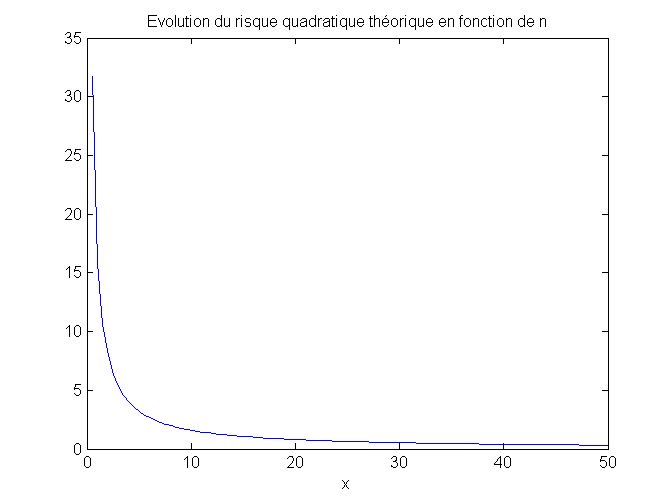
\includegraphics[scale=0.7]{sources/Q314-1.png}
			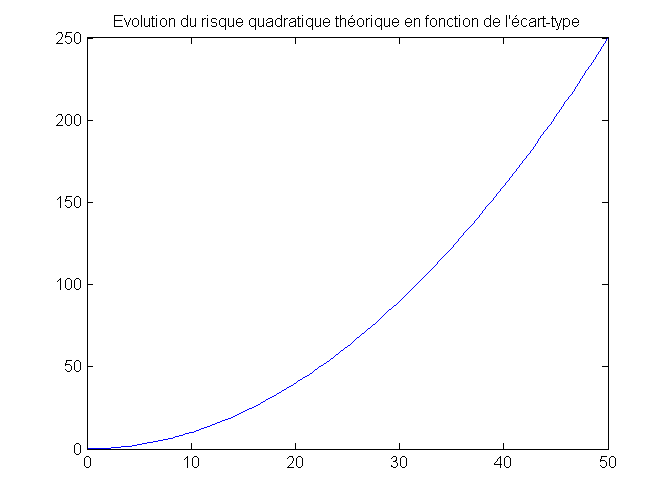
\includegraphics[scale=0.7]{sources/Q314-2.png}
			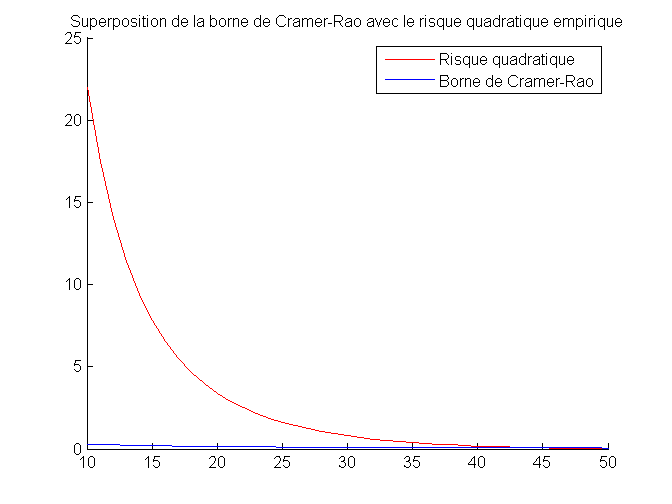
\includegraphics[scale=0.7]{sources/Q314-3.png}
		\end{center}
		\subsection{Loi de l'estimateur $\hat\sigma^2_n$}
			On a
			\begin{align*}
				\hat\sigma^2_n &= \frac{1}{n} \lVert (\mathbb{I} - \frac{1}{n}\textbf{1}\textbf{1}^T)X \rVert = \frac{1}{n} \sum\limits_{k=1}^n (X_k - \frac{1}{n}\sum\limits_{l=1}^n X_l)^2 = \lVert MX \rVert^2
			\end{align*}
			Avec
			\begin{align*}
				M = \frac{1}{\sqrt n}
				\left[
				\begin{array}{cccc}
					1-\frac{1}{n} & 1 & \cdots & 1 \\
					1 & \ddots & & \vdots \\
					\vdots & & \ddots & 1 \\
					1 &  \cdots & 1 & 1-\frac{1}{n}
				\end{array}
				\right]
			\end{align*}
			On a $MX = [M_1, \ldots, M_n]^T$ et
			\[ \forall k, M_k = \frac{1}{\sqrt n}[ (1-\frac{1}{n})X_k -\frac{1}{n}\sum\limits_{\substack{
            l=1\\
            l \neq k}}^n X_l ] \]
            On en déduit l'espérance et la variance de $\hat\sigma^2_n$\\
            \begin{align*}
            	\forall k, \mathbb{E}[M_k] &= \frac{1}{\sqrt n}[(1-\frac{1}{n})\mu - \frac{1}{n}\sum\limits_{\substack{
            	l=1\\
            	l \neq k}}^n \mu] = \frac{1}{\sqrt n}[ \mu - \frac{1}{n}\mu - \mu + \frac{1}{n}\mu ] = 0 \\
            	\forall k, Var{E}[M_k] &= \frac{1}{\sqrt n}[(1-\frac{1}{n})\sigma^2 - \frac{1}{n}\sum\limits_{\substack{
            	l=1\\
            	l \neq k}}^n \sigma^2] = \frac{\sigma^2}{n}(1-\frac{3}{n}+\frac{2}{n^2})
            \end{align*}
            Comme $\sigma^2 = \lVert M \rVert^2 = \sum\limits_{k=1}^n M_k^2$, alors \\
            $\sigma^2 \sim \chi^2(n)$, avec $\forall k, X_k \sim \mathcal{N}_{R}(0, \frac{\sigma^2}{n}(1-\frac{3}{n}+\frac{2}{n^2}))$
		\subsection{Biais de l'estimateur $\hat\sigma^2_n$}
		\subsection{Risque quadratique de l'estimateur $\hat\sigma^2_n$}
		\subsection{Tracé de l'évolution du risque quadratique de l'estimateur $\hat\sigma^2_n$}
			\begin{center}
				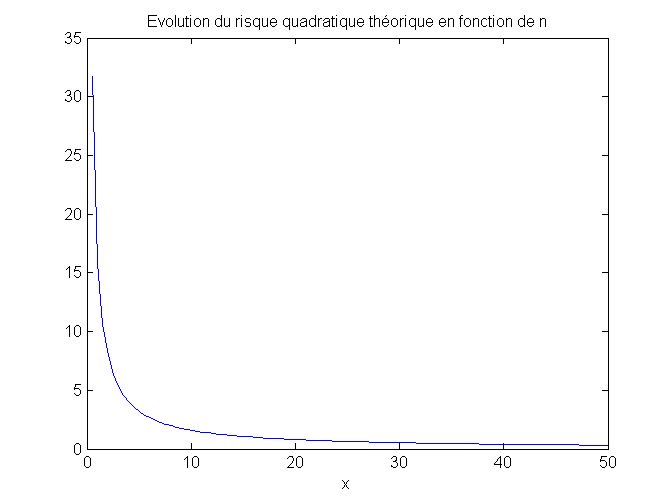
\includegraphics[scale=0.7]{sources/Q314-1.png}
				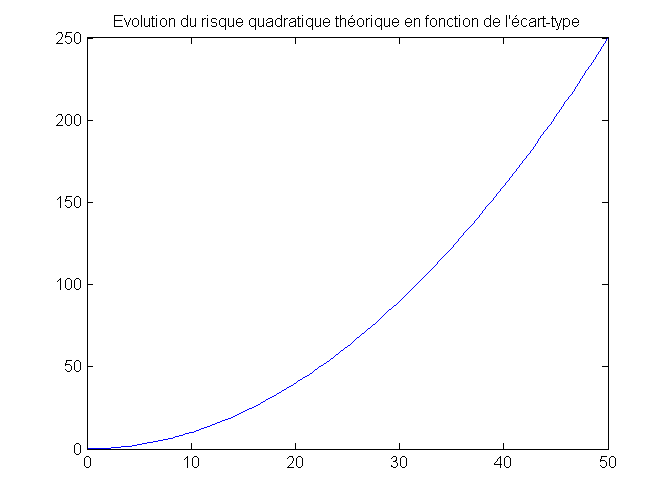
\includegraphics[scale=0.7]{sources/Q314-2.png}
				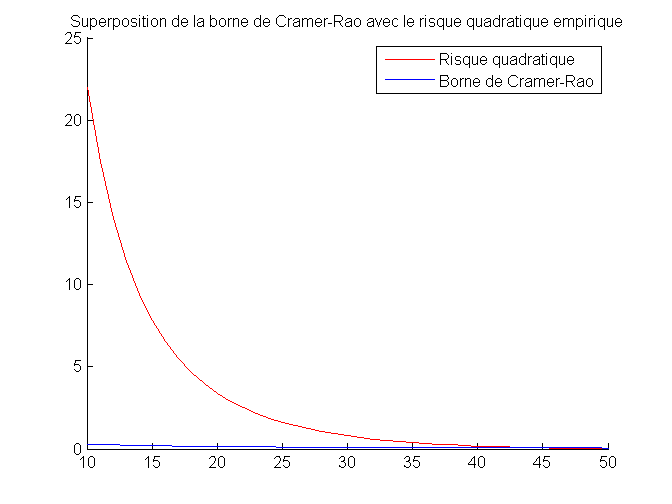
\includegraphics[scale=0.7]{sources/Q314-3.png}
			\end{center}


\end{document}
